\documentclass[10pt]{article}
\usepackage[utf8]{inputenc}
\usepackage[T1]{fontenc}
\usepackage[francais]{babel}
\usepackage[top=2.5cm, bottom=2.5cm, left=2.5cm, right=2.5cm]{geometry}
\usepackage{hyperref}   % Sommaire PDF
\usepackage{amsmath}    % Symboles mathématiques
\usepackage{amssymb}    % Flèches barrées
\usepackage{graphicx}   % Insertion d'images
\usepackage{multirow}   % Fusion de cellules de tableaux
\usepackage{float}      % Placement des figures
\usepackage{xcolor}     % Couleurs
\usepackage{eurosym}    % Symbole €
\usepackage{listings}	% Listings
\usepackage{alltt}		% Verbatim
\usepackage{makeidx}	% Index

% En-tête, pied-de-page
\usepackage{fancyhdr}
\pagestyle{fancy}
\renewcommand{\headrulewidth}{0pt}
\lhead{Bases de données\\2\up{ème} année}
\chead{}
\rhead{Rosine CICCHETI\\Lotfi LAKHAL\\Sebastien NEDJAR}
\lfoot{}
\cfoot{\thepage}
\rfoot{}
\makeindex

\begin{document}

\title{Bases de Données\\2\up{ème} année}
\author{Rosine CICCHETI, Lotfi LAKHAL, Sebastien NEDJAR}
\date{}

% Page de garde + page blanche
\maketitle
\setcounter{page}{0} \thispagestyle{empty} % Ne pas numéroter la page de garde

% Début du document
\newpage
Une application doit utiliser une base de données si :
	\begin{itemize}
		\item il y a un volume de données conséquent
		\item les données doivent être soumises à de nombreuses contraintes d'intégrité
		\item il y a plusieurs utilisateurs
		\item il y a besoin de la notion de transaction
	\end{itemize}
	
Le langage PL/SQL (Procedural Language/Structured Query Language) est un langage hôte qui accueille des instructions SQL.

\part{Structure d'un bloc PL/SQL}
	Il existe différents types de blocs :
		\begin{itemize}
			\item procédures
			\item fonctions
			\item packages
			\item blocs anonymes
		\end{itemize}

	Un programme PL/SQL a la structure suivante :\index{DECLARE}\index{BEGIN}\index{EXCEPTION}\index{END}
	\begin{alltt}
		\begin{tabbing}
			\emph{DECLARE}\=\\
						\><liste_declarations>\\
			\emph{BEGIN}\\
						\><liste_instructions>\\
			\emph{EXCEPTION}\\
						\><gestion_exceptions>\\
			\emph{END};
		\end{tabbing}
	\end{alltt}
	
\newpage
\part{Déclarations}
	On déclare des variables, des types, des exceptions développeurs et des curseurs.
	
	\section{Variables scalaires}
		Ce sont des variables simples dont le type est un des types proposés par Oracle : \emph{\texttt{VARCHAR2}}(n), \emph{\texttt{DATE}}, \emph{\texttt{NUMBER}}(m,n)\footnote{m chiffres, dont n décimales; par exemple 545.27 est un \emph{\texttt{NUMBER}}(5,2)}, \emph{\texttt{CHAR}}(n). On a aussi le type \emph{\texttt{BOOLEAN}} qui peut prendre trois valeurs : \emph{\texttt{TRUE}}, \emph{\texttt{FALSE}} et \emph{\texttt{NULL}}.\index{VARCHAR2}\index{DATE}\index{NUMBER}\index{CHAR}\index{BOOLEAN} \index{DEFAULT} \index{TRUE} \index{FALSE} \index{NULL}
		
		Une variable scalaire est déclarée ainsi : \texttt{<nomvariable> <nomtype> [}\emph{\texttt{NOT NULL}}\texttt{] [}\emph{\texttt{DEFAULT}}\texttt{ <valeur\_default>]}
		
		Au démarrage d'un programme, toutes les variables sont initialisées à \emph{\texttt{NULL}}, sauf celles qui ont une valeur par défaut. Les valeurs par défaut peuvent être des constantes, le résultat de calculs ou de fonction de calcul horizontal SQL (\emph{\texttt{UPPER}}, \emph{\texttt{LOWER}}, \emph{\texttt{LENGTH}},...), ou le contenu d'une autre variable. On peut aussi faire des déclarations par référence : déclarer une variable en lui donnant le même type qu'une autre variable ou qu'un attribut de la base.
		
		\paragraph{Exemple}
			\begin{alltt}
				\begin{tabbing}
					effectif\= \emph{NUMBER}(3,0); -- Nombre entier\\
					diplome\> \emph{VARCHAR2}(30) \=\emph{DEFAULT} 'DUT'; -- Chaine de caractère ayant 'DUT' comme valeur par défaut\\
					nb		\> \emph{NUMBER}(4,2) \>\emph{NOT NULL DEFAULT} 10; -- Nombre décimal ayant 10 comme valeur par défaut\\
					nb1 	\> \emph{NUMBER}(4,2) \>\emph{DEFAULT} nb; -- Nombre décimal prenant la valeur de nb\\
					nb2		\> nb\%\emph{TYPE} \>\emph{DEFAULT} nb*0.5; -- Variable du même type que nb, prenant comme valeur nb*0.5\\
					date_t	\> \emph{DATE}		\>\emph{DEFAULT SYSDATE}; -- Date, prenant comme valeur la date du jour (\emph{SYSDATE})
				\end{tabbing}
			\end{alltt}
	
		\paragraph{Exemple de déclaration par référence} \index{TYPE}
			\begin{alltt}
				\begin{tabbing}
					nb 	\=  \emph{NUMBER}(4,2) \=\emph{DEFAULT} 10;\\
					nb1 \>  nb\%\emph{TYPE};\\
					nom \>  ETUDIANT.NOM_ET \emph{TYPE};\\
					ville \>  ETUDIANT.VILLE\%\emph{TYPE};
				\end{tabbing}
			\end{alltt}
			
		Les déclarations par référence permettent une cohérence des déclarations des variables comparables, et une réduction de la maintenance des applications. Une variable déclarée par référence « hérite » de la clause \emph{\texttt{NOT NULL}}, mais pas de la valeur par défaut.
		
	\section{Variables composées}
		On peut utiliser des enregistrements ou des tableaux à une dimension.
		
		\subsection{Les enregistrements} \index{IS RECORD}
			\paragraph{Déclaration d'un type enregistrement}
				\begin{alltt}
					\begin{tabbing}
						\emph{TYPE} <nom_type> \emph{IS RECORD} (\=<nom_champ1> <type1> [\emph{NOT NULL}] [\emph{DEFAULT} <valeur_default1>]\\
																\> [, <nom_champ2> <type2> [\emph{NOT NULL}] [\emph{DEFAULT} <valeur_default2>]]\\
						<nom_variable> <nom_type>
					\end{tabbing}
				\end{alltt}
				
				On peut imbriquer les enregistrements.
				
				Pour manipuler les champs des variables enregistrement, on utilise \texttt{<nom\_variable>.<nom\_champ>}. Pour les variables enregistrement simples (non imbriquées), on peut faire des déclarations par référence avec \texttt{<nom\_variable> <nom\_type>\%>}\emph{\texttt{ROWTYPE}}, par exemple \texttt{<un\_etudiant> ETUDIANT\%}\emph{\texttt{ROWTYPE}}\index{ROWTYPE}
				
		\subsection{Les variables sculptures}
			Les tableaux sont à une dimension et les élements sont scalaires.
			
			\paragraph{Déclaration d'un type tableau} \index{IS TABLE OF} \index{INDEX BY} \index{BINARY\_INTEGER}
				\begin{alltt}
					\begin{tabbing}
						\emph{TYPE} \=<nom_type_tableau> \emph{IS TABLE OF} <nom_type | nom_var\%\emph{TYPE}>\\
									\>\emph{INDEX BY BINARY_INTEGER};\\
						<nom_variable> <nom_type_tableau>
					\end{tabbing}
				\end{alltt}
				
			Pour manipuler les élements du tableau, on utilise \texttt{<nom\_variable\_tableau>(index)}.
			
			En PL/SQL, les tableaux sont non denses (indices non consécutifs) et non bornés (taille dynamique).
			
			On dispose des primitives suivantes :
				\begin{itemize}
					\item \texttt{<nom\_variable>.}\emph{\texttt{EXISTS}}\texttt{(n)} renvoie vrai s'il existe un élément d'ordre $n$, faux sinon
					\item \texttt{<nom\_variable>.}\emph{\texttt{COUNT}} renvoie le nombre d'éléments existant dans le tableau
					\item \item \texttt{<nom\_variable>.}\emph{\texttt{FIRST}} renvoie l'indice du premier élément du tableau
					\item \item \texttt{<nom\_variable>.}\emph{\texttt{LAST}} renvoie l'indice du dernier élément du tableau
				\end{itemize}
				
			\texttt{tab.}\emph{\texttt{PRIOR}}\texttt{(tab.}\emph{\texttt{FIRST}}\texttt{)} et \texttt{tab.}\emph{\texttt{NEXT}}\texttt{(tab.}\emph{\texttt{LAST}}\texttt{)} renvoient \emph{\texttt{NULL}}.
			
		\subsection{Constantes}
			\texttt{<nom\_constante>} \emph{\texttt{CONSTANT}} \texttt{<nom\_type>:=<valeur>}
		
		\subsection{Exception}
			Seules les exceptions utilisateurs sont déclarées avec \texttt{<nom\_exception>} \emph{\texttt{EXCEPTION}}.
			
	\section{Instructions}
		\subsection{Affectation}
			\subsubsection{Affectation classique}
				On utilise \texttt{:=} pour donner une valeur à une variable.
				
				\paragraph{Exemple}
					On suppose qu'on a déclaré les variables et types nécessaires.
					\begin{alltt}
							nb:=100;
							nb1:=nb/2;
							adressse.ville:='Marseille';
							notes(3):=20;
					\end{alltt}
			\subsubsection{Affectation par requêtes}
				Pour cette affectation, la requête doit rendre au plus un résultat.
				
				\paragraph{Exemple}
					\begin{alltt}
						\begin{tabbing}
							\emph{DECLARE}\=\\
								\>Effectif \emph{NUMBER}(3,0);\\
								\>un_etudiant ETUDIANT\%\emph{ROWTYPE};\\
							\emph{BEGIN} \=\\
								\>\emph{SELECT}\= \emph{COUNT}(*) \emph{INTO} Effectif;\\
								\>\emph{FROM}\> ETUDIANT;\\
								\\
								\>\emph{SELECT}\> * \emph{INTO} un_etudiant\\
								\>\emph{FROM}\> ETUDIANT\\
								\>\emph{WHERE}\> NUM_ET=210;
							\emph{END}
						\end{tabbing}
					\end{alltt}
					
				La première affectation ne peut pas déclencher d'exception système (\texttt{Effectif=0} si la relation \texttt{ETUDIANT} est vide).
				La seconde peut déclencher l'exception système \texttt{NO\_DATA\_FOUND}.
				On peut spécifier plusieurs variables de réception pour une affectation.
				
		\subsection{Instructions conditionnelles}\index{IF}
			\begin{alltt}
				\begin{tabbing}
					\emph{IF}\= <condition> \emph{THEN}\\
						\>[\emph{BEGIN}]\\
						\><liste_instructions>\\
						\>[\emph{END}]\\
					\emph{ELSIF}\= <condition2> \emph{THEN}\\
						\><liste_instructions>\\
					\emph{ELSE}\=\\
						\><liste_instructions>\\
					\emph{END IF}
				\end{tabbing}
			\end{alltt}
			
			\texttt{<condition>} et \texttt{<condition2>} peuvent être des conditions liées par \texttt{AND}, \texttt{OR}, \texttt{NOT}, et on peut utiliser les prédicats SQL ou leur forme négative.
			
		\subsection{Itérations}
			\subsubsection{Boucle \emph{\texttt{FOR}}}\index{FOR}
				\begin{alltt}
					\begin{tabbing}
						\emph{FOR}\= <variable_de_parcours> \emph{IN} <borne_inf>..<borne_sup>\\
						\emph{BEGIN}\\
							\><liste_instructions>\\
						\emph{END LOOP};
					\end{tabbing}
				\end{alltt}
		
				\texttt{<variable\_de\_parcours>} ne doit pas être initialisée.
			
			\subsubsection{Boucle \emph{\texttt{WHILE}}}\index{WHILE}
				\begin{alltt}
					\begin{tabbing}
						\emph{WHILE} \= <condition> \emph{LOOP}\\
							\> <liste_instructions>\\
						\emph{END LOOP};
					\end{tabbing}
				\end{alltt}
				
				\newpage
				\paragraph{Exemple : parcours d'un tableau}
				\begin{alltt}
					\begin{tabbing}
						numero := Notes.\emph{FIRST}\\
						\emph{WHILE} \= numero \emph{IS NOT NULL LOOP}\\
							\> <liste_instructions>\\
							\> numero:=Notes.\emph{NEXT}(numero)\\
						\emph{END LOOP};
					\end{tabbing}
				\end{alltt}
				
			\subsubsection{Boucles répeter/jusqu'à (\emph{\texttt{EXIT WHEN}}}\index{EXI WHEN}
				\begin{alltt}
					\begin{tabbing}
						\emph{LOOP}\=\\
							\><instructions>\\
							\>\emph{EXIT WHEN} <condition_sortie>\\
						\emph{END LOOP};
					\end{tabbing}
				\end{alltt}
				
				\paragraph{Exemple : parcours d'un tableau}
					\begin{alltt}
						\begin{tabbing}
							numero:=NOTES.\emph{FIRST};\\
							\emph{LOOP}\=\\
								\><instructions>\\
								\>numero:=Notes.\emph{NEXT}(numero);\\
								\>\emph{EXIT WHEN} numero \emph{IS NULL}\\
							\emph{END LOOP};
						\end{tabbing}
					\end{alltt}
		\subsection{Autres instructions}
			\begin{itemize}
				\item pour lever une exception utilisateur déclarée : \emph{\texttt{RAISE}} \texttt{<nom\_exception>}\index{RAISE}
				\item pour « ne rien faire » (terminer le programme proprement) : \emph{\texttt{NULL}}\index{NULL}
			\end{itemize}
			
	\section{Les curseurs}
		Dans l'univers des bases de données, on manipule les tuples sous forme d'ensemble. Dans l'univers de la programmation, on manipule les tuples enregistrement par enregistrement. Pour lier les deux, on utilise des curseurs. On peut voir un curseur comme le résultat d'une requête. On le déclare par \emph{\texttt{CURSOR}} \texttt{<nom\_curseur>} \emph{\texttt{IS}} \texttt{<requete>;}\index{CURSOR}
			\begin{figure}[H]
				\begin{center}
					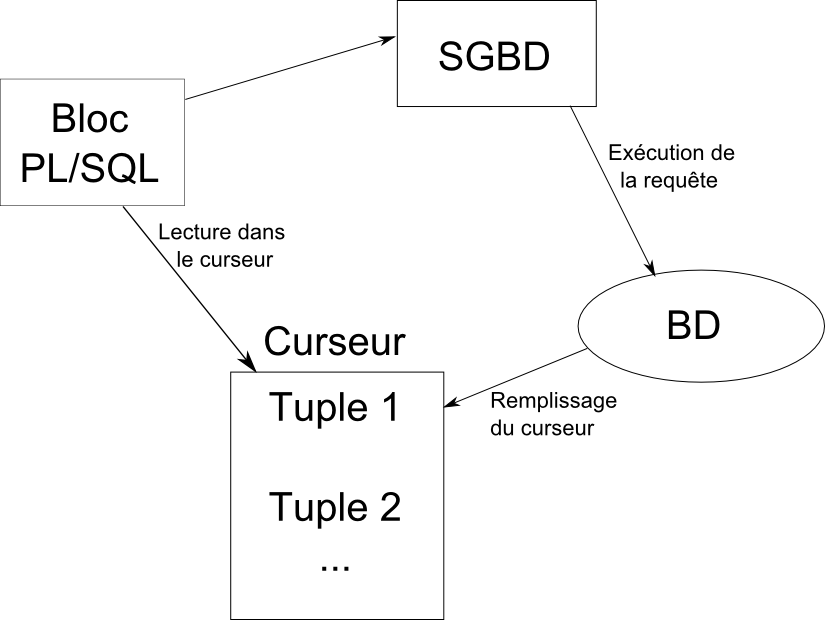
\includegraphics[width=\textwidth]{images/RepresentationCurseur.png}
				\end{center}
				\caption{Représentation d'un curseur}
			\end{figure}
			
			\paragraph{Exemple} On a besoin de récupérer, dans un bloc PL/SQL, la liste des étudiants de 2\up{ème} année. Dans la base, on a la relation \texttt{ETUDIANT(}\underline{\texttt{NUM\_ET}}\texttt{, NOM\_ET, PRENOM\_ET, ..., ANNEE)}.
				\begin{alltt}
					\begin{tabbing}
						\emph{DECLARE} \=\\
							\>\emph{CURSOR} Et2 \emph{IN} \=\emph{SELECT}\= NUM_ET, PRENOM_ET\\
												\>\>\emph{FROM} ETUDIANT\\
												\>\>\emph{WHERE} ANNEE=2\\
												\>\>\emph{ORDER BY} NOM_ET, PRENOM_ET
					\end{tabbing}
				\end{alltt}

        \subsection{Ordres de déclaration des curseurs}
            \begin{itemize}
                \item \emph{\texttt{OPEN}} \texttt{<nom\_curseur>;}\index{OPEN}\\
                    La requête de définition du curseur est exécutée et le curseur est rempli.
                \item \emph{\texttt{CLOSE}} \texttt{<<nom\_curseur>;}\index{CLOSE}\\
                    La zone mémoire nécessaire est liberée.
                \item \emph{\texttt{FETCH}} \texttt{<nom\_curseur>} \emph{\texttt{INTO}} \texttt{<nom\_variable>;}\index{FETCH}\\
                    Retourne un enregistrement dans \texttt{<nom\_variable>}.
            \end{itemize}

            \texttt{<nom\_variable>} peut être :
            \begin{itemize}
                \item une liste de variables scalaires
                \item une variable enregistrement qui peut avoir la même structure que le curseur
            \end{itemize}

            \newpage
            \paragraph{Exemple : on déclare Et2}
                \begin{alltt}
                    \begin{tabbing}
nom ETUDIANT_NOM\%\emph{TYPE};\\
prenom ETUDIANT_PRENOM\%\emph{TYPE};\\
-- OU\\
etudiant Et2\%\emph{ROWTYPE};
\\
\emph{FETCH} Et2 \emph{INTO} nom, prenom;\\
-- OU\\
\emph{FETCH} Et2 \emph{INTO} etudiant;\\
\\
nom:=\emph{UPPER}(nom)\\
prenom:=\emph{PRENOM}(prenom)\\
-- OU\\
etudiant.NOM_ET:=\emph{UPPER}(etudiant.NOM_ET)
                    \end{tabbing}
                \end{alltt}

        \subsection{Propriétés des curseurs}
            \begin{itemize}
                \item \texttt{<nom\_curseur>\%}\emph{\texttt{FOUND}} (ou \emph{\texttt{NOTFOUND}}) rend \emph{\texttt{TRUE}} si le dernier \emph{\texttt{FETCH}} a renvoyé un résultat
                \item \texttt{<nom\_curseur>\%}\emph{\texttt{ISOPEN}} rend vrai si le curseur est ouvert
                \item \texttt{<nom\_curseur>\%}\emph{\texttt{ROWCOUNT}} rend le nombre d'enregistrements retournées par les \emph{\texttt{FETCH}}. Cette propriété vaut 0 à l'ouverture du curseur.
            \end{itemize}

            \paragraph{Exemple : on utilise le curseur Et2 et la variable enregistrement}
                \begin{alltt}
                    \begin{tabbing}
\emph{BEGIN}\=\\
    \>\emph{OPEN} \= Et2;\\
    \>\emph{FETCH}\> Et2 \emph{INTO} etudiant;\\
    \>\emph{WHILE}\> Et2\%\emph{FOUND LOOP}\\
        \>\><instructions>\\
        \>\>\emph{FETCH} Et2 \emph{INTO} etudiant;\\
    \>\emph{END LOOP};\\
    \>\emph{CLOSE} Et2;\\
\emph{END};
                    \end{tabbing}
                \end{alltt}

            \paragraph{Exemple : avec une boucle \emph{\texttt{EXIT WHEN}}}
                \begin{alltt}
                    \begin{tabbing}
\emph{BEGIN}\=\\
    \>\emph{OPEN} \= Et2;\\
    \>\emph{LOOP}\\
        \>\>\emph{FETCH} Et2 \emph{INTO} etudiant;\\
        \>\><instructions>\\
        \>\>\emph{EXIT WHEN} Et2\%\emph{NOTFOUND};\\
    \>\emph{END LOOP};\\
    \>\emph{CLOSE} Et2;\\
\emph{END};
                    \end{tabbing}
                \end{alltt}
                
			\paragraph{Exemple}
				Dans une base, on a la relation \texttt{ETUDIANT(}\underline{\texttt{NUM\_ET}}\texttt{,...,DEPT\#)}. On vient de créer la relation \texttt{EFF\_DEPT(}\underline{\texttt{NUM\_DEPT}}\texttt{,EFF)} qui est vide. On va écrire un bloc permettant de remplir cette relation à partir des données de \texttt{ETUDIANT}.
				
				\begin{alltt}
					\begin{tabbing}
						\emph{DECLARE}\=\\
							\>\emph{CURSOR} \=E_D \emph{IS} \=\emph{SELECT} \=\emph{COUNT}(*)\\
															\>\>\emph{FROM}\>ETUDIANT\\
															\>\>\emph{GROUP BY} DEPT;\\
							\>E\>ED\%\emph{ROWTYPE};\\
						\emph{BEGIN}\\
							\>\emph{OPEN} E_D;\\
							\>\emph{FETCH} E_D \emph{INTO} E;\\
							\>\emph{WHILE} \=E_D\%\emph{FOUND LOOP}\\
								\>\>\emph{INSERT INTO} \= EFF_DEPT(NUM_DEPT,EFF)\\
								\>\>\>\emph{VALUES}(E.DEPT, E.EFF);\\
								\>\>\emph{FETCH} E_D \emph{INTO} E;\\
							\>\emph{END LOOP};\\
							\>\emph{CLOSE} E_D;
						\emph{END};
					\end{tabbing}
				\end{alltt}
				
				On suppose qu'on a \texttt{EFF\_DEPT(}\underline{\texttt{NUM\_DEPT}}\texttt{, EFF, EFF\_AN1, EFF\_AN2)}. Ces effectifs peuvent être calculés à partir de la relation \emph{ETUDIANT}.
				
				\begin{alltt}
					\begin{tabbing}
						\emph{DECLARE}\=\\
							\>\emph{CURSOR} \= ET1_D \emph{IS} \=\emph{SELECT} \=DEPT, \emph{COUNT}(*) F1\\
									\>\>\emph{FROM}\>ETUDIANT\\
									\>\>\emph{WHERE}\>ANNEE=1\\
									\>\>\emph{GROUP BY} DEPT;\\
							\>E1\>ET1_D\%\emph{ROWTYPE}\\
						\emph{BEGIN}\\
							\>\emph{OPEN} ET1_D;\\
							\>\emph{FETCH} ET1_D \emph{INTO} E1;\\
							\>\emph{WHILE} \= ET1_D\%\emph{FOUND LOOP}\\
								\>\>\emph{UPDATE} \=EFF_DEPT\\
								\>\>\>\emph{SET}\>EFF_AN1=E1.F1\\
								\>\>\>\emph{WHERE}\>NUMDEP=E1.DEPT;\\
								\>\>\emph{FETCH} ET1_D \emph{INTO} E1;\\
							\>\emph{END LOOP};
							\>\emph{CLOSE ET1_D};
						\emph{END};
					\end{tabbing}
				\end{alltt}

		\subsection{Curseurs paramétrés}
			On peut paramétrer les constantes de sélection d'un curseur.
			
			\paragraph{Exemple}
				\begin{alltt}
					\begin{tabbing}
						\emph{CURSOR} \=EFF_AN(An ETUDIANT, AN\%\emph{TYPE}) \emph{IS} \=\emph{SELECT} \=DEPT, \emph{COUNT}(*) Nb\\
									\>\emph{FROM}\>ETUDIANT\\
									\>\emph{WHERE}\>ANNEE=An\\
									\>\emph{GROUP BY} DEPT;\\
						E \>EFF_AN\%\emph{ROWTYPE};\\
						\emph{OPEN} \>EF_AN(1);
					\end{tabbing}
				\end{alltt}
				
		\subsection{Parcours automatique d'un curseur}
			Les particularités du parcours automatique sont qu'il n'y a pas de variable de parcours, pas de \emph{\texttt{OPEN/CLOSE}}, et pas de \emph{\texttt{FETCH}}.
			
				\begin{alltt}
					\begin{tabbing}
						\emph{FOR} <nom_variable> \emph{IN} <nom_curseur>\\
						\emph{LOOP} \=\\
							\><instructions>\\
						\emph{END LOOP};
					\end{tabbing}
				\end{alltt}
				
				\paragraph{Exemple}
					\begin{alltt}
						\begin{tabbing}
							\emph{DECLARE}\=\\
								\>\emph{CURSOR} CM \emph{IS}\\
							\emph{BEGIN}\>\\
								\>\emph{FOR} \=vCM \emph{IN} CM \emph{LOOP}\\
									\>\><instructions>\\
								\>\emph{END LOOP};\\
							\emph{END}
						\end{tabbing}
					\end{alltt}
					
	\section{Les exceptions}
		Elles sont utilisateur ou système, anonymes ou nomées.
		
		\subsection{Exceptions système nommées}
			Une dizaine d'exception est nommée par exemple : \emph{\texttt{NO\_DATA\_FOUND}}, \emph{\texttt{TOO\_MANY\_ROWS}}, \emph{\texttt{ZERO\_DIVIDE}}, \emph{\texttt{INVALID\_CURSOR}}, ...
			
		\subsection{Exceptions système anonymes}\index{sqlcode} \index{sqlerm}
			C'est le cas de la majorité des exceptions Oracle. Elles ont un code (négatif). Les fonctions \emph{\texttt{sqlcode}} et \emph{\texttt{sqlerm}} renvoient respectivement le code et le message de l'erreur.
			
		\subsection{Exceptions utilisateur anonymes}\index{RAISE\_APPLICATION\_ERROR}
			Elles sont réservées aux triggers et blocs stockés. On ne les déclare pas dans \emph{\texttt{DECLARE}}. On les déclenche avec :
			\begin{alltt}
				\emph{IF} <condition> \emph{THEN RAISE_APPLICATION_ERROR}(<code>, <message>); \emph{END IF};
			\end{alltt}
			
			\texttt{<code>} est dans l'intervalle $\left[-20 999; -20 000\right]$.
			
		\subsection{Traitement des exceptions}\index{WHEN}
			Toutes les exceptions, sauf les exceptions utilisateur anonymes, doivent être traitées dans la partie \emph{\texttt{EXCEPTION}}.
			
			\begin{alltt}
				\begin{tabbing}
					\emph{EXCE}\=\emph{PTION}\\
						\>\emph{WHEN} <nom_exception> \emph{THEN} <traitement>;\\
						\>\emph{WHEN} <exception1> \emph{OR} <exception2> \emph{THEN} <traitement>;\\
						\>\emph{WHEN}\=\emph{OTHERS THEN}\\
							\>\>\emph{IF} sqlcode = <code> \emph{THEN}\\
							\>\>\emph{END IF};\\
				\end{tabbing}
			\end{alltt}
			
	\section{Les différents types de blocs}
	 Les blocs, procédures, fonctions et blocs anonymes peuvent être imbriquéess les uns das les autre.
	 
	 	\subsection{Procédures}
	 		\begin{alltt}
	 			\begin{tabbing}
	 				\emph{PROCEDURE}\= <nom_procedure> (\=<nom_parametre1> <mode_parametre1>  <type_parametre1>\\
	 												\>\>[,<nom_parametre2> <mode_parametre2> <type_parametre2>...]) \emph{IS}\\
	 					\><declarations_locales>\\
	 					\>\emph{BEGIN}\=\\
	 						\>\><instructions>\\
	 				\emph{END} <nom_procedure>;
	 			\end{tabbing}
	 		\end{alltt}
	 		
	 		\texttt{<mode\_parametre>} peut être \emph{\texttt{IN}}, \emph{\texttt{OUT}} ou \emph{\texttt{IN OUT}}.
	 		
	 		\paragraph{Exemple : fonction qui permet de formatter le nom et prénom}
	 			\begin{alltt}
	 				\begin{tabbing}
	 					\emph{PROCEDURE} \= Formatter (\=nom \emph{IN OUT} ETUDIANT.NOM_ET\%\emph{ROWTYPE},\\
	 												\>\>prenom \emph{IN OUT} ETUDIANT\%\emph{ROWTYPE}) \emph{IS}\\
	 						\>nom:=\emph{UPPER}(nom);\\
	 						\>prenom:=\emph{INITCAP}(prenom);\\
	 					\emph{END} Formatter;
	 				\end{tabbing}
	 			\end{alltt}
	 			
	 	\subsection{Fonction}
	 		\begin{alltt}
	 			\begin{tabbing}
	 				\emph{FUNCTION} \=<nom_fonction> (\=<nom_parametre1> <mode_parametre1> <type_paramatre1>\\
	 												\>\>[<nom_parametre2> <mode_parametre2> <type_parametre2>...])\\
	 												\>\>\emph{RETURN} <type_retour> \emph{IS}\\
	 					\><instructions>\\
	 					\>\emph{RETURN}(<valeur_retour>);\\
	 				\emph{END} <nom_fonction>;
	 			\end{tabbing}
	 		\end{alltt}
	 		
	 	\subsection{Procédures stockées et fonctions stockées}\index{CREATE} \index{REPLACE}
	 		La procédure ou fonction est stockée comme un objet Oracle et décrit dans des tables système (jusqu'à son code). On peut alors l'appeler depuis n'importe quel autre bloc.
	 		
	 		\begin{alltt}
	 			\begin{tabbing}
	 				\emph{CREATE}\=[\emph{OR REPLACE}] \emph{PROCEDURE | FUNCTION} <nom_bloc>(<parametres>) [\emph{RETURN} <type_retour>] \emph{IS} ...\\
	 				\><instructions>\\
	 				\emph{END} <nom_bloc>;
	 			\end{tabbing}
	 		\end{alltt}

        \subsection{Blocs imbriqués}
            \begin{figure}[H]
                \begin{center}
                    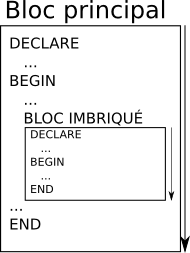
\includegraphics{images/BlocImbrique.png}
                \end{center}
                \caption{Portée des variables}
            \end{figure}


            \paragraph{Exemple de l'intérêt des blocs imbriqués}
                On suppose qu'on doit faire un \emph{\texttt{INSERT}} dans une relation 1, puis dans une relation 2.

                \subparagraph{Hypothèse} :le 1\up{er} \emph{\texttt{INSERT}} lève une exception; toutes les instructions suivantes (dont le 2\up{ème} \emph{\texttt{INSERT}}) ne sont pas évaluées. En utilisant des blocs imbriquées, on peut poursuivre l'exécution.

                \begin{alltt}
                    \begin{tabbing}
\emph{DECLARE}\=\\
    \><declarations>\\
\emph{BEGIN}\=\\
    \><instructions>\\
    \>\emph{DECLARE}\=\\
        \>\><declarations>\\
    \>\emph{BEGIN}\=\\
        \>\><instructions>\\
        \>\>\emph{INSERT} ...\\
    \>\emph{EXCEPTION}\\
    \>\emph{END}\\
    \>\emph{INSERT} ... \\
\emph{END}
                    \end{tabbing}
                \end{alltt}

    \section{Les triggers (déclencheurs)}
        Les triggers sont aussi appelés « règles ECA » (Évènement/Condition/Action).
        \begin{itemize}
            \item[E] Quand un évènement survient sur la base de données
            \item[C] Si une condition est vérifiée
            \item[A] Alors l'action est exécutée
        \end{itemize}

        \paragraph{Intérêts}
            \begin{itemize}
                \item le même trigger peut être déclenché par plusieurs programmes, ce qui rend le code plus modulaire
                \item on peut automatiquement déclencher la vérification des contraintes dynamiques, des actions ou des alertes (seuil atteint,...)
                \item permet de propager automatiquement une mise à jour des données
            \end{itemize}

        \subsection{Partie Évènement}
            Un évènement est la détection par le système d'un ordre SQL (à l'exception de \emph{\texttt{SELECT}}) par un utilisateur (humain ou programme).

            Les ordres SQL peuvent être des ordres :
                \begin{itemize}
                    \item du LMD : \emph{\texttt{INSERT}, \texttt{DELETE}, \texttt{UPDATE}}
                    \item du LDD : \emph{\texttt{CREATE}, \texttt{ALTER}}
                    \item du LCD : \emph{\texttt{GRANT}, \texttt{REVOQUE}}
                \end{itemize}

            \subsection{Chronologie d'un trigger}
                \begin{figure}[H]
                    \begin{tabular}{*{4}{p{4cm}}}
                        Détection de l'ordre SQL déclencheur du trigger & Exécution du trigger de type \emph{\texttt{BEFORE}} & Exécution de l'ordre SQL & Exécution du trigger de type \emph{\texttt{AFTER}} \\
                        \hline
                        |t1 & |t2 & |t3 & |t4
                    \end{tabular}
                    \caption{Chronologie d'un trigger}
                \end{figure}

                \paragraph{Remarque}
                    \begin{itemize}
                        \item un trigger permettant le contrôle ou la mise en forme de données est forcément de type \emph{\texttt{BEFORE}} car il doit vérifier/formatter les données avant leur insertion
                        \item un trigger effectuant la propagation d'une mise à jour est forcément de type \emph{\texttt{AFTER}} car il faut être sûr que l'ordre SQL déclencheur a bien été exécuté
                    \end{itemize}

            \subsection{Granularité des triggers LMD}
                Un trigger LMD peut être orienté ensemble (exécuté une seule fois pour tous les tuples concernés par l'ordre SQL déclencheur), ou orienté tuple (exécuté pour chaque tuple concerné).

                \begin{figure}[H]
                    \begin{tabular}{*{4}{p{4cm}}}
                        & & \multicolumn{2}{c}{$\Downarrow n+1 \Leftarrow$} \\
                       Ordre SQL LMD de l'utilisateur & Lecture des tuples concernés par l'ordre SQL & Exécution du trigger de type \emph{\texttt{BEFORE}} pour le tuple $n$ & Exécution de l'ordre SQL pour le tuple $n$ \\
                       \hline
                        |t1 & |t2 & |t3 & |t4
                    \end{tabular}
                    \caption{Chronologie d'un trigger orienté tuple de type \emph{\texttt{BEFORE}}}
                \end{figure}

            \subsection{Informations véhiculées par un évènement}
                Il est possible d'utiliser \emph{\texttt{OLD}} et \emph{\texttt{NEW}} pour accéder à l'ancien et au nouveau tuple manipulé par un trigger LMD orienté tuple.

                \paragraph{Exemple}
                    \begin{alltt}
                        \begin{tabbing}
\emph{UPDATE}\=NOTATION\\
\emph{SET}\>MOY_TEST=15\\
\emph{WHERE}\>CODE='BD' \emph{AND} NUM_ET=2401;
                        \end{tabbing}
                    \end{alltt}

                On suppose que la moyenne de cet étudiant en BD était 12.
                \begin{itemize}
                    \item \emph{\texttt{OLD}}\texttt{.NUM\_ET=}\emph{\texttt{NEW}}\texttt{.NUM\_ET=24401}
                    \item \emph{\texttt{OLD}}\texttt{.CODE=}\emph{\texttt{NEW}}\texttt{.CODE='BD'}
                    \item \emph{\texttt{OLD}}\texttt{.MOY\_TEST=12} et \emph{\texttt{NEW}}\texttt{.MOY\_TEST=15}
                \end{itemize}

                Pour \emph{\texttt{INSERT}}, \emph{\texttt{NEW}}\texttt{.attribut=}nouvelle valeur de l'attribut, et \emph{\texttt{OLD}}\texttt{.attribut=}\emph{\texttt{NULL}}.

                Pour \emph{\texttt{DELETE}}, \emph{\texttt{OLD}}\texttt{.attribut}=valeur avant la suppression, et \emph{\texttt{NEW}}\texttt{.attribut=}\emph{\texttt{NULL}}.

            \subsection{Partie Condition}
                Pour les triggers LMD orientés tuples, où une seule relation est concernée, les conditions (dans \emph{\texttt{WHEN}}) sont des combinaisons booléennes de conditions simples (comme les conditions de \emph{\texttt{WHERE}}).

                \paragraph{Remarque} pas de jointure imbriquée
                \begin{figure}[H]
                    \begin{tabular}{*{7}{p{2cm}}}
                        Ordre LMD & Lecture des tuples concernés & Évaluation de la condition pour le 1\up{er} tuple & Exécution du trigger pour le 1\up{er} tuple & Exécution de la requête pour le 1\up{er} tuple & Évaluation de la condition pour le 2\up{ème} tuple & Exécution de la requête pour le 2\up{ème} tuple \\
                       \hline
                        |t1 & |t2 & |t3 & |t4 & |t5 & |t6 & |t7\\
                        && Condition vraie pour le 1\up{er} tuple && Condition fausse pour le 2\up{ème} tuple
                    \end{tabular}
                    \caption{Chronologie de la partie condition}
                \end{figure}

            \subsection{Partie Action}
                \begin{itemize}
                    \item Jamais de \emph{\texttt{COMMIT}} ou de \emph{\texttt{ROLLBACK}} car le trigger est déclenché au cours d'une transaction qu'il n'a jamais le droit de terminer ou de défaire
                    \item Pour les triggers LMD orientés tuples, on ne peut pas faire de mise à jour sur la relation concernée (table en mutation)
                    \item On peut utiliser \emph{\texttt{IF [INSERTING | DELETING | UPDATING]}}
                    \item Enchainement de triggers

                    \begin{figure}[H]
                        \begin{center}
                        \end{center}
                        \caption{Enchainement de triggers}
                    \end{figure}
                \end{itemize}

            \subsection{Syntaxe}
                \begin{alltt}
                    \begin{tabbing}
\emph{CREATE} [\emph{OR REPLACE}] \emph{TRIGGER} <nom_trigger>\\
\emph{BEFORE | AFTER} <element_delencheur> \\
[\emph{FOR EACH ROW}]\\
[\emph{WHEN} <condition>]\\
[\emph{DECLARE} ...]\\
[\emph{BEGIN}]\\
    <instructions>\\
[\emph{END};]
                    \end{tabbing}
                \end{alltt}

                \paragraph{Exemple} mise à jour de l'effectif des professeurs dans \emph{\texttt{DEPNT}}\texttt{(}\underline{\texttt{NOM\_DEP}}\texttt{,Eff\_P)}
                \begin{alltt}
                    \begin{tabbing}
\emph{CREATE OR REPLACE TRIGGER} MajEff\\
\emph{AFTER INSERT ON} PROF\\
\emph{FOR EACH ROW}\\
\emph{WHEN NEW}.DEP \emph{IS NOT NULL}\\
-- Partie Action\\
\emph{UPDATE} DEPNT\\
\emph{SET} EFF_P=EFF_P+1\\
\emph{WHERE} NOM_DEP=\emph{:NEW}.DEP
                    \end{tabbing}
                \end{alltt}

                Pour exécuter une opération lors des mises à jour et suppression :
                \begin{alltt}
                    \begin{tabbing}
\emph{CREATE OR REPLACE TRIGGER} MajEff\\
\emph{AFTER INSERT OR UPDATE OF} DEP \emph{OR DELETE ON} PROF\\
\emph{FOR EACH ROW}\\
\emph{WHEN NEW}.DEP \emph{IS NOT NULL OR OLD}.DEP \emph{IS NULL}\\
-- Partie Action\\
\emph{IF}\=\emph{INSERTING THEN}\\
    \>  \emph{UPDATE} DEPNT\\
    \>  \emph{SET} EFF_P=EFF_P+1\\
    \>  \emph{WHERE} NOM_DEP=\emph{:NEW}.DEP\\
\emph{ELIF}\=\emph{DELETING THEN}\\
    \>\emph{UPDATE} DEPNT\\
    \>\emph{SET} EFF_P=EFF_P-1\\
    \>\emph{WHERE} NOM_DEP=\emph{:OLD}.DEP\\
\emph{ELSE}\=\\
    \>\emph{UPDATE} DEPNT\\
    \>\emph{SET} EFF_P=EFF_P-1\\
    \>\emph{WHERE} NOM_DEP=\emph{:OLD}.DEP\\
    \>\emph{UPDATE} DEPNT\\
    \>\emph{SET} EFF_P=EFF_P+1\\
    \>\emph{WHERE} NOM_DEP=\emph{:NEW}.DEP\\
\emph{END}
                    \end{tabbing}
                \end{alltt}
\newpage
\part*{Index}
\tableofcontents
\newpage
\listoftables
\listoffigures
\renewcommand{\indexname}{Liste des mots-clefs PL/SQL} \printindex
\end{document}
